\TieudeT{PHONG TỎA VẬT LÍ 12 - VẬT LÍ NHIỆT}
\subsubsection*{PHẦN I. Thí sinh trả lời câu hỏi từ câu 1 đến câu 18. Mỗi câu hỏi thí sinh chỉ chọn một phương án}
\setcounter{ex}{0}
\begin{ex}
	Phát biểu sau đây nói về chuyển động của phân tử là \textbf{không} đúng?
	\choice
	{\True Chuyển động của phân tử là do lực tương tác phân tử gây ra}
	{Các phân tử chuyển động không ngừng}
	{Các phân tử chuyển động càng nhanh thì nhiệt độ càng cao}
	{Các phân tử khí không dao động quanh vị trí cân bằng}
	\loigiai{}
\end{ex}

\begin{ex}
	Phát biểu nào sau đây nói về lực tương tác phân tử là \textbf{không} đúng?
	\choice
	{Lực tương tác phân tử chỉ đáng kể khi các phân tử ở rất gần nhau}
	{Lực hút phân tử có thể lớn hơn lực đẩy phân tử}
	{\True Lực hút phân tử không thể lớn hơn lực đẩy phân tử}
	{Lực hút phân tử có thể bằng lực đẩy phân tử}
	\loigiai{}
\end{ex}

\begin{ex}
	Phát biểu nào sau đây \textbf{sai} khi nói về cấu tạo chất?
	\choice
	{Các chất được cấu tạo từ các nguyên tử, phân tử}
	{Các nguyên tử, phân tử chuyển động nhiệt càng nhanh thì nhiệt độ của vật càng cao}
	{Các nguyên tử, phân tử đồng thời hút nhau và đẩy nhau}
	{\True Các nguyên tử, phân tử càng xa nhau thì lực liên kết phân tử càng mạnh}
	\loigiai{}
\end{ex}

\begin{ex}
	Các tính chất nào sau đây sai khi nói về tính chất của các phân tử chất rắn?
	\choice
	{Dao động quanh vị trí cân bằng xác định}
	{Lực tương tác phân tử mạnh}
	{Có hình dạng và thể tích xác định}
	{\True Có lực hút phân tử lớn hơn lực đẩy phân tử}
	\loigiai{}
\end{ex}

\begin{ex}
	Vật nào sau đây \textbf{không} có cấu trúc tinh thể?
	\choice
	{\True Chiếc cốc thủy tinh}
	{Hạt muối ăn}
	{Viên kim cương}
	{Miếng thạch anh}
	\loigiai{}
\end{ex}

\begin{ex}
	So sánh nhiệt độ nóng chảy và nhiệt độ đông đặc của nước. Phát biểu nào sau đây đúng?
	\choice
	{Nhiệt độ nóng chảy cao hơn nhiệt độ đông đặc}
	{Nhiệt độ nóng chảy thấp hơn nhiệt độ đông đặc}
	{Nhiệt độ nóng chảy có thể cao hơn, cũng có thể thấp hơn nhiệt độ đông đặc}
	{\True Nhiệt độ nóng chảy bằng nhiệt độ đông đặc}
	\loigiai{}
\end{ex}

\begin{ex}
	Phát biểu nào sau đây là \textbf{sai} khi nói về sự nóng chảy và sự đông đặc?
	\choice
	{Các chất khác nhau sẽ nóng chảy (hay đông đặc) ở nhiệt độ khác nhau}
	{Đối với một chất nhất định, nếu nóng chảy ở nhiệt độ nào thì sẽ đông đặc ở nhiệt độ ấy}
	{\True Nhiệt độ của một chất sẽ tăng dần trong quá trình nóng chảy và giảm dần trong quá trình đông đặc}
	{Phần lớn các chất nóng chảy (hay đông đặc) ở một nhiệt độ nhất định}
	\loigiai{}
\end{ex}

\begin{ex}
	Trường hợp nào sau đây \textbf{không} liên quan đến sự nóng chảy và đông đặc?
	\choice
	{Ngọn nến vừa tắt}
	{Ngọn nến đang cháy}
	{Cục nước đá lấy ra khỏi tủ lạnh}
	{\True Ngọn đèn dầu đang cháy}
	\loigiai{}
\end{ex}

\begin{ex}
	Hiện tượng vào mùa đông ở các nước vùng băng tuyết thường xảy ra sự cố vỡ đường ống nước là do
	\choice
	{tuyết rơi nhiều đè nặng thành ống}
	{\True thể tích nước khi đông đặc tăng lên gây ra áp lực lớn lên thành ống}
	{trời lạnh làm đường ống bị cứng giòn và rạn nứt}
	{ống nước để lâu nên bị giòn}
	\loigiai{}
\end{ex}

\begin{ex}
	Tốc độ bay hơi của chất lỏng \textbf{không} phụ thuộc vào yếu tố nào sau đây?
	\choice
	{\True Thể tích của chất lỏng}
	{Gió}
	{Nhiệt độ}
	{Diện tích mặt thoáng của chất lỏng}
	\loigiai{}
\end{ex}

\begin{ex}
	Các bình ở hình vẽ đều chứa cùng một lượng nước và được đặt trong cùng một phòng. Phát biểu nào sau đây là đúng?
	\begin{center}
		\begin{tikzpicture}[draw=Mapcolor, very thick, line join=round,thick]
			\fill [cyan!50] (-0.75,1) rectangle ++ (1.5,-1);
			\draw [rounded corners=1pt](-0.25,2.5) -- (-0.25,2) -- (-0.75,2) -- (-0.75,0) -- (0.75,0) -- (0.75,2) -- (0.25,2) -- (0.25,2.5);
			\draw node [below] at (0,0) {$A$};
			\begin{scope}[shift={(3,0)}]
				\fill [cyan!50] (-1,0.8) rectangle ++ (2,-0.8);
				\draw [rounded corners=1pt] (-1,1.5) -- (-1,0) -- (1,0) -- (1,1.5);
				\draw node [below] at (0,0) {$B$};
			\end{scope}
			\begin{scope}[shift={(6,0)}]
				\fill [cyan!50] (-0.5,1.5) rectangle ++ (1,-1.5);
				\draw [rounded corners=1pt] (-0.5,2) -- (-0.5,0) -- (0.5,0) -- (0.5,2);
				\draw node [below] at (0,0) {$C$};
			\end{scope}
		\end{tikzpicture}
	\end{center}
	\choice
	{Nước trong bình A cạn chậm nhất}
	{Nước trong bình B cạn chậm nhất}
	{\True Nước trong bình C cạn chậm nhất}
	{Nước trong ba bình cạn như nhau}
	\loigiai{}
\end{ex}

\begin{ex}
	Trong suốt thời gian sôi, nhiệt độ của chất lỏng
	\choice
	{tăng dần lên}
	{giảm dần đi}
	{khi tăng khi giảm}
	{\True không thay đổi}
	\loigiai{}
\end{ex}

\begin{ex}
	Hiện tượng nào sau đây \textbf{không} phải là sự ngưng tụ?
	\choice
	{Hơi nước trong các đám mây sau một thời gian sẽ tạo thành mưa}
	{Khi hà hơi vào mặt kính cửa sổ sẽ xuất hiện những hạt nước nhỏ làm mờ kính}
	{Sự tạo thành giọt nước đọng trên lá cây vào ban đêm}
	{\True Nước mưa trên đường nhựa biến mất khi Mặt Trời lại xuất hiện sau cơn mưa}
	\loigiai{}
\end{ex}

\begin{ex}
	Mây được tạo thành từ
	\choice
	{nước bay hơi}
	{khói}
	{nước đông đặc}
	{\True hơi nước ngưng tụ}
	\loigiai{}
\end{ex}

\begin{ex}
	Tại sao khi cầm vào vỏ bình ga mini khi vừa sử dụng xong ta thường thấy có một lớp nước rất mỏng trên đó?
	\choice
	{Do hơi nước từ tay ta bốc ra}
	{Nước từ trong bình ga thấm ra}
	{\True Do vỏ bình ga lạnh hơn nhiệt độ môi trường nên hơi nước trong không khí ngưng tụ trên đó}
	{Hơi nước trong không khí đông đặc khi tiếp xúc với bề mặt lạnh của bình ga}
	\loigiai{}
\end{ex}

\begin{ex}
	Một vật có khối lượng riêng $\rho$. Nếu khối lượng của vật là $m$ thì thể tích của vật là
	\choice
	{\True $\dfrac{m}{\rho}$}
	{$\dfrac{\rho}{m}$}
	{$\rho m$}
	{$\sqrt{\rho m}$}
	\loigiai{}
\end{ex}

\begin{ex}
	Gọi $N_A$ là hằng số Avogadro. Một chất rắn có khối lượng mol $M$ và khối lượng riêng $\rho$ thì thể tích không gian trung bình của mỗi phân tử chiếm trong chất rắn đó là
	\choice
	{$\dfrac{\rho}{MN_A}$}
	{$\dfrac{\rho N_A}{M}$}
	{\True $\dfrac{M}{\rho N_A}$}
	{$\dfrac{\rho M}{N_A}$}
	\loigiai{}
\end{ex}

\begin{ex}
	Một chất lỏng có khối lượng mol $M$, thể tích mol $V_m$, khối lượng riêng $\rho$, khối lượng của một phân tử $m_0$. Với hằng số Avogadro $N_A$ thì mối liên hệ nào sau đây \textbf{không} đúng?
	\choice
	{$m_0=\rho V_m$}
	{$M=\rho V_m$}
	{$M=m_0N_A$}
	{\True $m_0=\dfrac{\rho V_m}{N_A}$}
	\loigiai{}
\end{ex}
\subsubsection*{PHẦN 2. Thí sinh trả lời từ câu 1 đến câu 4. Trong mỗi ý a), b), c), d) ở mỗi câu, thí sinh chọn đúng hoặc sai.}
\setcounter{ex}{0}
\begin{ex}
	Một vật ở thể rắn có thể tích và hình dạng xác định.
	\choiceTF[t]
	{Ở thể rắn, các nguyên tử, phân tử dính chặt thành một khối}
	{\True Lực tương tác giữa các nguyên tử, phân tử chất rắn rất mạnh}
	{\True Các nguyên tử, phân tử chỉ có thể dao động xung quanh các vị trí cân bằng xác định}
	{Các nguyên tử, phân tử chỉ có thể dao động xung quanh các vị trí cân bằng không cố định}
	\loigiai{
		\begin{itemchoice}
			\itemch Vì giữa các nguyên tử, phân tử có khoảng cách chứ không dính chặt thành một khối
			\itemch 
			\itemch 
			\itemch Vì đây là tính chất của thể lỏng
		\end{itemchoice}
	}
\end{ex}
\begin{ex}
\impicinpar{Sinh viên ngày xưa thường dùng thiết bị gọi là "sục điện" để đun nước. Vào thời kỳ đó, hầu hết sinh viên đều có điều kiện kinh tế hạn chế, nên việc sắm một chiếc ấm đun nước điện là khá tốn kém. Sục điện là một lựa chọn vừa rẻ tiền, nhỏ gọn, linh hoạt, tiện dụng và đặc biệt tiết kiệm thời gian. Một đầu sục điện là một sợi kim loại xoắn kép - thường là nhôm, nối giữa hai đầu dây nhôm là dây điện có phích cắm. Lúc đun thì thả cái lõi kim loại đó vào trong cốc nhựa, xô nhựa chứa nước rồi cắm điện. Một sinh viên dùng chiếc sục điện có ghi $2500 \ W-220 \ V$ để đun $10$ lít nước ở $20^\circ C$ chứa trong một xô nhựa. Ở điện cắm sục có hiệu điện thế là $220\ V$ . Nước thu được $90 \%$ nhiệt do dây xoắn kép tỏa ra. Biết khối lượng riêng của nước là $1000 \ kg/m^3$, nhiệt dung riêng của nước là $4200\ J/kg.K$. Nhiệt độ sôi của nước là $100^\circ C$.}
	{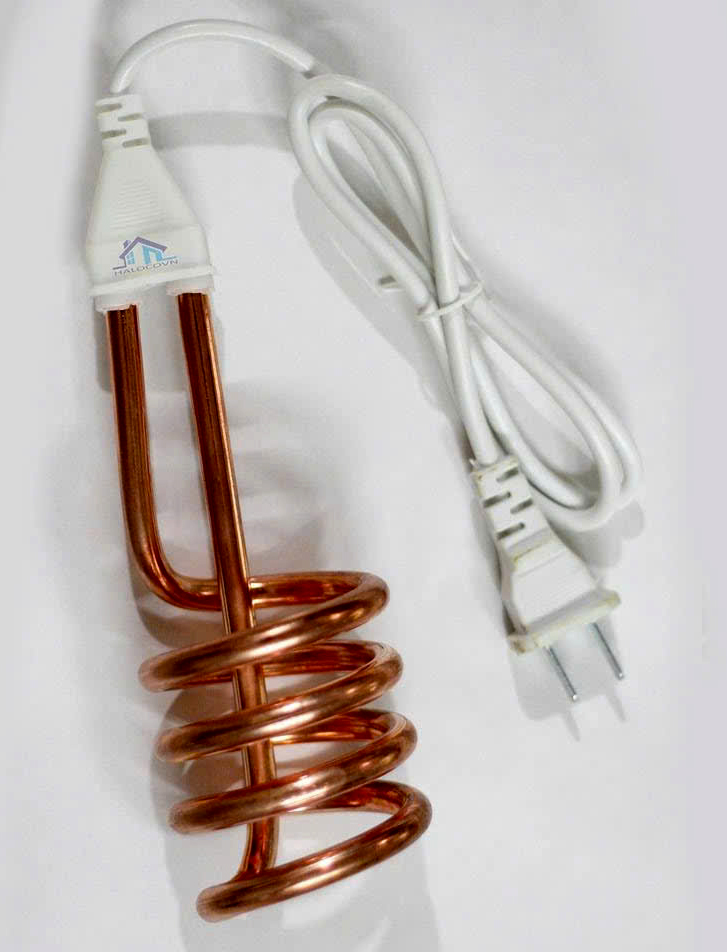
\includegraphics[width=4 cm]{Images/De36KhanhLyBai1}}
	\choiceTF[t]
	{\True Thiết bị này đã biến đổi trực tiếp điện năng thành nhiệt năng }
	{Để đun nước trong xô đến sôi, sinh viên đó cần đun trong $20,2$ phút}
	{Muốn có nước tắm ở $40^\circ C$, sinh viên đó cần pha thêm $40$ lít nước ở $20^\circ C$ vào $10$ lít nước sôi}
	{ Đây là thiết bị đun nước rất an toàn và đảm bảo sức khỏe nên được sinh viên chọn dùng phổ biến}
	\loigiai{
		
		\begin{itemchoice}
			\itemch Thiết bị này đã biến đổi trực tiếp điện năng thành nhiệt năng.
			\itemch Nhiệt lượng cung cấp cho nước tính theo công thức :$Q=\mathcal{P}.t =m.c.\Delta t$.
			\itemch  Phương trình cân bằng nhiệt: $Q_{\text{tỏa}}=Q_{\text{thu}}$ nên ta có\\
			$10.4200.(100-30)=m.4200.(40-20)\Rightarrow m=30\ kg \Rightarrow V=30\ (l)$
			\itemch  Đây là thiết bị đun nước không an toàn.
		\end{itemchoice}
	}
\end{ex}


\begin{ex}
	Đồ thị hình bên biểu diễn sự thay đổi nhiệt độ theo thời gian khi một chất lỏng nào đó đông đặc.
	\begin{center}
		\begin{tikzpicture}[draw=Mapcolor, very thick, >=latex']
			\draw [dotted] (0,0) grid (6,4);
			\draw [->](0,0) -- (7.5,0) node [above] {Thời gian (phút)};
			\draw [->](0,0) -- (0,5) node [right] {Nhiệt độ $(^\circ C)$};
			\foreach \x in {2,4,...,12}{
			\draw (\x/2,0.1) -- (\x/2,-0.1) node [below] {\x};
			}
			\foreach \y in {20,40,...,80}{
			\draw (0.1,\y/20) -- (-0.1,\y/20) node [left] {\y};
			}
			\draw (0,4) -- (2,4) -- (6,1);
		\end{tikzpicture}
	\end{center}
	\choiceTF[t]
	{\True Chất lỏng đông đặc ở $80^\circ C$}
	{Quá trình giảm nhiệt độ diễn ra trong $4$ phút}
	{Trung bình mất $0,5$ phút để nhiệt chất lỏng hạ xuống $1$ độ}
	{Sau thời gian $9$ phút thì nhiệt độ là $40^\circ C$}
	\loigiai{
	\begin{itemchoice}
		\itemch Vì nhiệt độ ban đầu $80^\circ C$ không đổi
		\itemch Quá trình diễn ra trong 8 phút.
		\itemch Trong quá trình giảm nhiệt độ, chất đang ở trạng thái rắn.
		\itemch $\dfrac{\Delta t(^\circ C)}{\Delta \tau (ph)} = \text{const} \Rightarrow \dfrac{20-80}{12-4} = \dfrac{x-80}{9-4} \Rightarrow x = 42,5^\circ C$.
	\end{itemchoice}
	}
\end{ex}

\begin{ex}
	Nước ở thể lỏng có khối lượng mol là $18\ g/mol$ và khối lượng riêng là $1\ g/cm^3$.
	\choiceTF[t]
	{\True Khối lượng của $1,5$ lít nước ở thể lỏng là $1,5\ kg$}
	{Thể tích của $5$ mol nước ở thể lỏng là $3,6\ cm^3$}
	{Số phân tử có trong $270\ g$ nước ở thể lỏng là $4,01.10^{22}$}
	{\True Giả sử nước ở thể lỏng có các phân tử nước cách đều nhau, mỗi phân tử nằm ở tâm của một khối lập phương nhỏ, các khối lập phương nhỏ liền kề chạm nhau nhưng không chồng lấn lên nhau thì độ dài của cạnh của các khối lập phương nhỏ đó là $3,1.10^{-10}\ m$}
	\loigiai{
		\begin{itemchoice}
			\itemch Vì $m = V.D = 1,5\ kg$
			\itemch .Vì $V = \dfrac{nM}{D} = \dfrac{5.18}{1} = 90\ cm^3$
			\itemch Sai vì $N = n.N_A = \dfrac{270}{18}.6,02.10^{23} = 9,03.10^{24}$
			\itemch Vì Thể tích $1$ mol nước là $V = \dfrac{M}{D} = \dfrac{18}{1} = 18\ cm^3$ Trung bình $1$ phân tử nước chiếm thể tích là $V = \dfrac{18}{6,02.10^{23}} \approx 3.10^{-23}\ cm^3$ Thể tích hình lập phương $V = a^3 \Rightarrow a = \sqrt[3]{V} = \sqrt[3]{3.10^{-23}} \approx 3,1.10^{-8}\ cm = 3,1.10^{-10}\ m$
		\end{itemchoice}
	}
\end{ex}
\subsubsection*{PHẦN 3. Thí sinh trả lời từ câu 1 đến câu 6.}
\setcounter{ex}{0}
\begin{ex}% Câu 1
	Cho bảng thay đổi nhiệt độ nóng chảy của chất rắn như sau
	\begin{center}
		
		
		\begin{tabular}{|>{\raggedright\arraybackslash}m{4cm}|
				>{\centering\arraybackslash}m{1cm}|
				>{\centering\arraybackslash}m{1cm}|
				>{\centering\arraybackslash}m{1cm}|
				>{\centering\arraybackslash}m{1cm}|
				>{\centering\arraybackslash}m{1cm}|
				>{\centering\arraybackslash}m{1cm}|}
			\hline
			\textbf{Thời gian (phút)} & $0$ & $2$ & $4$ & $6$ & $8$ & $10$ \\
			\hline
			\textbf{Nhiệt độ ($^\circ$C)} & $20$ & $40$ & $60$ & $80$ & $80$ & $85$ \\
			\hline
		\end{tabular}
	\end{center}
	Sau thời gian bao nhiêu phút thì chất rắn bắt đầu nóng chảy?
	\shortans[oly]{$6$}
	\loigiai{}
\end{ex}

\begin{ex}% Câu 2
	Bảng dưới đây ghi nhiệt độ nóng chảy (đông đặc) của một số chất
	\begin{center}
	\begin{tabular}
		{|>{\raggedright\arraybackslash}m{3cm}|
			>{\centering\arraybackslash}m{2cm}|
			>{\centering\arraybackslash}m{2cm}|
			>{\centering\arraybackslash}m{2cm}|
			>{\centering\arraybackslash}m{2cm}|
			>{\centering\arraybackslash}m{2cm}|
			>{\centering\arraybackslash}m{2cm}|}
		\hline
		\textbf{Chất}	& Đồng & Vàng & Bạc & Nước & Thủy ngân & Rượu \\
		\hline
		\textbf{Nhiệt độ $(^\circ C)$}	& $1093$ & $1063$ & $960$ & $0$ & $-39$ & $-114$ \\
		\hline
	\end{tabular}
	
	\end{center}
	Ở nhiệt độ $25^\circ C$, có bao nhiêu chất ở thể rắn?
	\shortans[oly]{$3$}
	\loigiai{}
\end{ex}

\begin{ex}% Câu 3
	Khối lượng mol của muối ăn là $58,5\ g/mol$. Mỗi phân tử muối ăn (NaCl) có khối lượng là $x.10^{-23}\ g$. Giá trị của $x$ bằng bao nhiêu (làm tròn kết quả đến chữ số hàng phần mười)?
	
	\shortans[oly]{$9,7$}
	\loigiai{
	$m_0 = \dfrac{M}{N_A} = \dfrac{58,5}{6,02.10^{23}} \approx 9,7.10^{23}$.
	}
\end{ex}

\begin{ex}% Câu 4
	Biết nước có khối lượng mol $18\ g/mol$ và khối lượng riêng $1\ g/cm^3$. Một giọt sương hình cầu đường kính $5\ mm$ có chứa $N.10^{21}$ phân tử nước. Giá trị của $N$ bằng bao nhiêu (làm tròn kết quả đến chữ số hàng phần mười)?
	\shortans[oly]{$2,2$}
	\loigiai{
	\begin{itemize}
		\item $N = n.N_A = \dfrac{m}{M}.N_A = \dfrac{D.V}{M}.N_A = \dfrac{D. \dfrac{4}{3}\pi R^3.N_A}{M} =\dfrac{1. \dfrac{4}{3}\pi 0.25^3.6,02.10^{23}}{18} \approx 2,2.10^{21}$.
	\end{itemize}
	}
\end{ex}

\begin{ex}% Câu 5
	Biết calcium có khối lượng mol $40\ g/mol$ và khối lượng riêng $1,55\ g/cm^3$. Giả thiết trong tinh thể calcium chứa các nguyên tử là những quả cầu chiếm $74\%$ thể tích tinh thể, còn lại là khe rỗng. Bán kính nguyên tử calcium theo giả thiết này bằng bao nhiêu $pm$ (làm tròn kết quả đến chữ số hàng đơn vị)?
	
	\shortans[oly]{$196$}
	\loigiai{
	\begin{itemize}
		\item Thể tích 1 $mol$ canxi: $ V_m = \dfrac{M}{D} = \dfrac{40}{1,55} = \dfrac{800}{31}\ cm^3$.
		\item Thể tích 1 nguyên tử canxi: $V_{Ca} = \dfrac{V_m.0,74}{N_A} = \dfrac{4}{3}\pi R^3 \Rightarrow R \approx 1,96.10^{-8}\ cm = 196\ pm$.
		
	\end{itemize}
	}
\end{ex}

\begin{ex}% Câu 6
	Nước thể lỏng có khối lượng mol là $18\ g/mol$ và khối lượng riêng là $1\ g/cm^3$. Coi một phân tử nước dạng hình cầu có đường kính là $3.10^{-10}\ m$ và khoảng cách giữa Trái Đất và Mặt Trời là $149,6$ triệu $km$. Nếu lấy các phân tử trong $0,1\ ml$ nước thể lỏng xếp một hàng sát nhau thì tạo ra một đoạn thẳng dài gấp khoảng bao nhiêu lần khoảng cách từ Trái Đất đến Mặt Trời (làm tròn kết quả đến chữ số hàng đơn vị)?
	
	\shortans[oly]{$7$}
	\loigiai{
	\begin{itemize}
		\item Số phân tử nước: $N = n.N_A = \dfrac{m}{M}.N_A = \dfrac{\rho .V}{M}.N_A = \dfrac{0,1.1}{18}.6,02.10^{23} = \dfrac{6,02.10^{23}}{180}$ phân tử.
		\item $\dfrac{N.d}{149,6.10^9} = \dfrac{\dfrac{6,02.10^{23}}{180}.3.10^{-10}}{149,6.10^9} \approx 7$.
	\end{itemize}
	}
\end{ex}
